% replace all text with your own text.
% in this template few examples are mention
\chapter{Methodology}
\label{ch:method} % Label for method chapter
\section{Dataset Description and Data Exploration}
The diabetes data set is originated from kaggle \citep{dataset}. The dataset contains 2000 patients and their corresponding 9 unique attributes. The nine attributes that are used for the prediction of diabetes are `Pregnancies`, 
`Glucose`, `BloodPressure`, `SkinThickness`, `Insulin`, `BMI`, `DiabetesPedigreeFunction`, 
`Age`, `Outcome`. The `Outcome` attribute is taken as a dependent or target variable, and the remaining eight attributes are taken as independent feature variables. 
 \begin{table}[ht!]
    \centering
    \caption{Dataset attributes and their data types}
    \begin{tabular}{llll}
 & Attribute & Description & Type \\
0 & Pregnancies & Number of times pregnant & Numeric \\
1 & Glucose & Plasma glucose concentration & Numeric \\
2 & BloodPressure & Diastolic blood pressure & Numeric \\
3 & SkinThickness & Triceps skinfold thickness & Numeric \\
4 & Insulin & 2-hour serum insulin & Numeric \\
5 & BMI & Body mass index & Numeric \\
6 & DiabetesPedigreeFunction & Diabetes pedigree function & Numeric \\
7 & Age & Age (years) & Numeric \\
8 & Outcome & Diabetes diagnose results (0: Negative, 1: Positive) & Nominal \\
\end{tabular}

    \label{tab:table-03-data-info}
\end{table}

\begin{figure}[ht]
    \centering    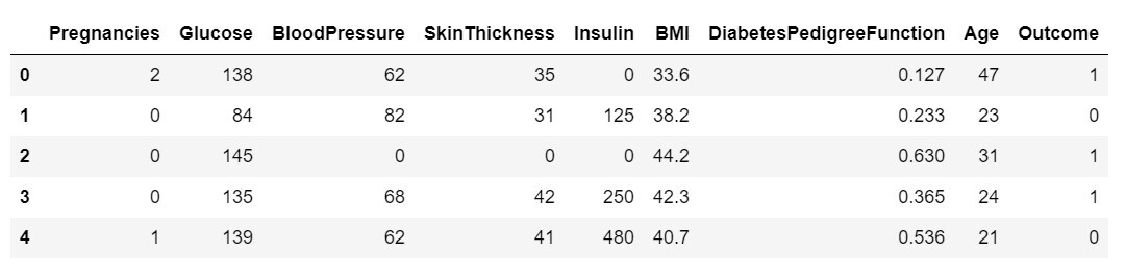
\includegraphics[scale=0.8]{figures/data_top5.pdf}
    \caption{Top 5 patients data}
    \label{fig:capture_b}
\end{figure}

The diabetes attribute `Outcome` is a categorical feature which consists of binary value where 0 means non-diabetes, and 1 implies diabetes. There are no null values for all attributes but there are zero values for few attributes which needs to be handled.

\subsection{Data Distribution using Histograms}
Fig~\ref{fig:capture_d} gives a better feel than the raw numbers and percentiles of the distributions of our numerical attributes. It shows how each feature and label is distributed along different ranges which further confirms the need for scaling. Next, wherever you see discrete bars, it basically means that each of these is actually a categorical variable. We will need to handle these categorical variables before applying Machine Learning. Our outcome labels have two classes, 0 for no disease and 1 for disease. 
\begin{figure}[ht]
    \centering    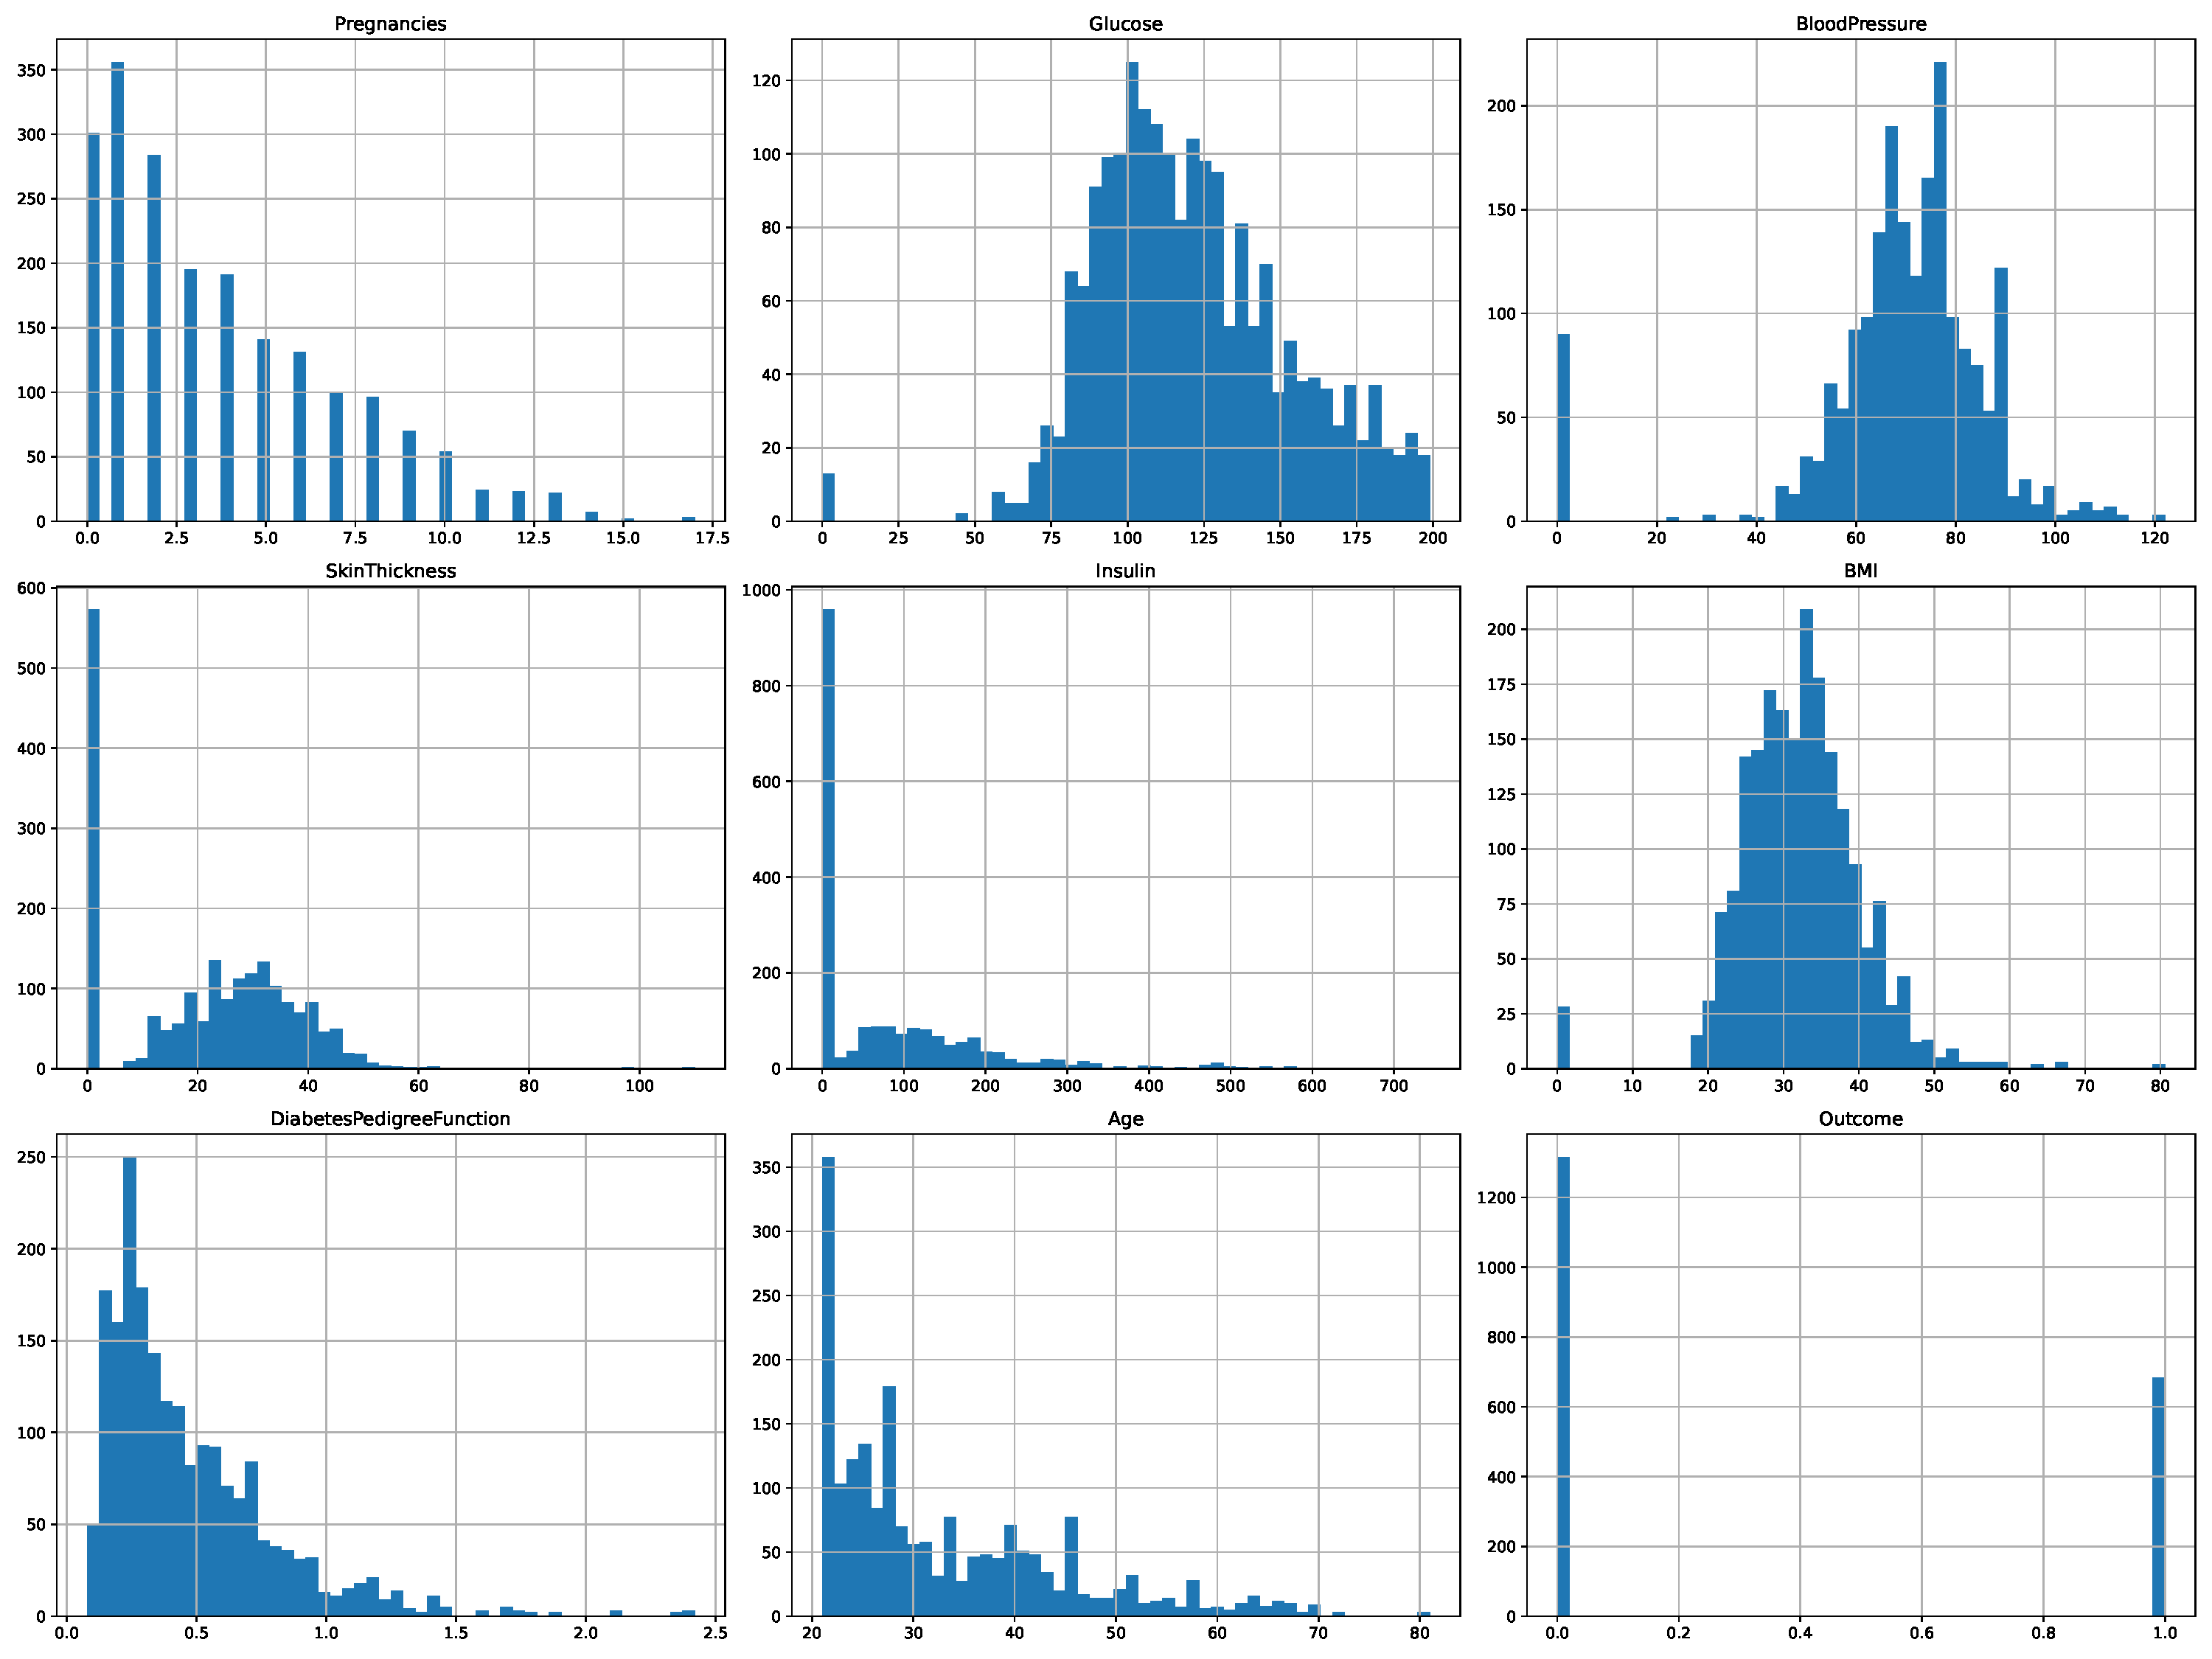
\includegraphics[scale=0.3]{figures/data_attr_distribution.pdf}
    \caption{Data Distribution for each attribute}
    \label{fig:capture_d}
\end{figure}

\subsection{Correlation Matrix}
\label{subsec:corr_matrix}
A correlation matrix is a powerful tool for data analysis. It is a statistical technique used to evaluate the relationship between two variables in a dataset. It provides a correlation coefficient for each cell. The correlation coefficient value remains in the range between -1 and 1.

The correlation coefficient value -1 indicates notable negative linear correlation. The coefficient value 1 indicates notable positive linear correlation. The coefficient value 0 indicates no linear correlation.

A correlation matrix helps summarize data, identify patterns, and make decisions based on relationships between attributes. It helps us to gain insights for building better machine learning models by understanding which attributes are correlated.

\begin{figure}[ht]
    \centering    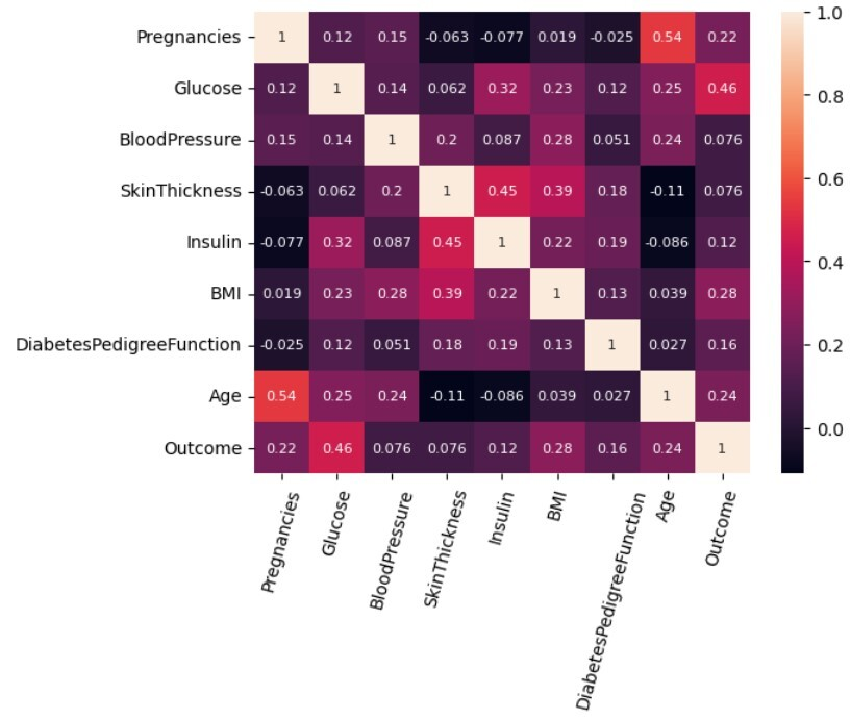
\includegraphics[scale=0.8]{figures/data_correlation.pdf}
    \caption{Correlation Matrix}
    \label{fig:capture_c}
\end{figure} 

Here, we have to check the attributes correlated to target feature `Outcome`. In Fig~\ref{fig:capture_c}, `Glucose` has highest correlation coefficient value - 0.46 and `BMI` has 0.28, `Age` has 0.24 and `Pregnancies` has 0.22 compare to other attributes.

\subsection{Bar plot for Outcome class}
Fig~\ref{fig:capture_e} shows that the data is biased towards data points having outcome value as 0 which means that diabetes was not present actually. The number of non-diabetics is almost twice the number of diabetic patients.

Out of the 2000 instances, 1316 are associated with non-diabetic patients, while the remaining 684 pertain to diabetic patients. Therefore, it is essential to split the data efficiently for training and testing the model to ensure optimal results.
\begin{figure}[ht]
    \centering    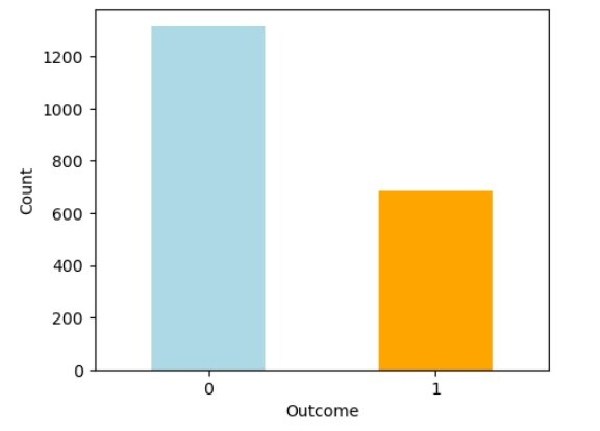
\includegraphics[scale=0.8]{figures/data_distribution.pdf}
    \caption{Distribution of Outcome (0s and 1s)}
    \label{fig:capture_e}
\end{figure}


\section{Data Preprocessing}
Data preprocessing helps to transform data used to built a model which gives higher performance metrics. This process performs various functions like handling missing values, normalization and feature selection to improve the quality of data.

\subsection{Missing Values Identification}
There are no null values for all attributes. However, Fig~\ref{fig:capture_b} illustrates instances of zero values for attributes which are irrelevant and need to handled. Table~\ref{tab:table-01-missing-values} shows the number of zero values for each attribute before imputation and after performing imputation.

 \begin{table}[ht!]
    \centering
    \caption{The number of zero missing values in dataset}
    \begin{tabular}{lrrrrr}
Attributes & No.of missing values (Zero) \\
Pregnancies & 301 \\
Glucose & 13 \\
BloodPressure & 90 \\
SkinThickness & 573 \\
Insulin & 956 \\
BMI & 28 \\
DiabetesPedigreeFunction & 0 \\
Age & 0 \\
\end{tabular}


    \label{tab:table-01-missing-values}
\end{table}

Here, we have observed numerous attributes with zero values, impacting the data quality. We replaced the zero values with the corresponding mean values using simpleimputer.

Fig~\ref{fig:capture_b} and Fig~\ref{fig:capture_f} shows the top five patients data. If you compare these figures, Fig~\ref{fig:capture_f} indicates that zero values in Fig~\ref{fig:capture_b} was replaced with mean for each attribute. Now, there are no missing values either null or zero values in each attribute.

\begin{figure}[ht]
    \centering    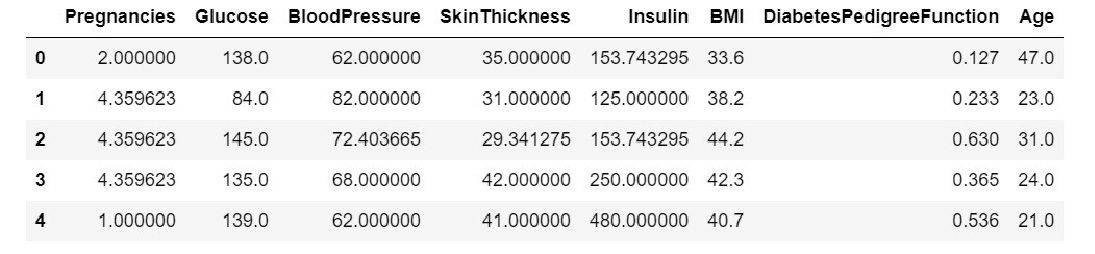
\includegraphics[scale=0.8]{figures/data_info_after_imputer.pdf}
    \caption{Top 5 patients data after handling missing values}
    \label{fig:capture_f}
\end{figure}

\subsection{Feature Selection based on Correlation Coefficient}
After handling missing values, the correlation coefficient is calculated in this method which correlates with the output and input attributes. This was discussed under section~\ref{subsec:corr_matrix}. We have created a Table~\ref{tab:table-02-corr_matrix} to show correlation coefficient values of each attribute towards target attribute.

 \begin{table}[ht!]
    \centering
    \caption{The correlation coefficient values}
    \begin{tabular}{lrr}
 & Correlation Coefficient & Correlation Coefficient after imputation \\
Pregnancies & 0.224437 & 0.249883 \\
Glucose & 0.458421 & 0.488020 \\
BloodPressure & 0.075958 & 0.174481 \\
SkinThickness & 0.076040 & 0.205527 \\
Insulin & 0.120924 & 0.207696 \\
BMI & 0.276726 & 0.282182 \\
DiabetesPedigreeFunction & 0.155459 & 0.155459 \\
Age & 0.236509 & 0.236509 \\
\end{tabular}

    \label{tab:table-02-corr_matrix}
\end{table}

We used 0.2 as a cut-off for relevant attributes. Hence   `BloodPressure` and `DiabetesPedigreeFunction` features are removed. `Pregnancies`, `Glucose`, `SkinThickness`, `Insulin`, `BMI`, and `Age` are our most relevant six input attributes.

\subsection{Data Normalization}
Normalization refers to the process of scaling and transforming numeric features to a standard scale or distribution. Feature scaling is a technique to standardize or normalize the range of independent features or variables of a dataset. The goal of feature scaling is to ensure that all features contribute equally to the learning process, preventing certain features from dominating others based on their scale. In Table~\ref{tab:table-02-corr_matrix}, we can see that `Glucose` and `Outcome` have a 0.49 correlation coefficient. Hence these are highly correlated. After completing data preprocessing, we have total 2000 instances.

\section{Dataset Split into Train and Test Data}
After data cleaning and preprocessing, the dataset becomes ready to train and test. We are using test split method to split data randomly into the training and testing set. Here, I am partitioning the data into a training set comprising 70\% and a test set comprising 30\%.

\section{Model Implementation}
This is the important phase which includes model building for diabetes prediction.

\subsection{Logistic Regression}
It is used for classification task where the goal is to predict the probability that an instance belongs to a given class or not.

\begin{algorithm}
    \caption{Diabetes Prediction using Logistic Regression}
    \label{algo:algo_lr}
    \begin{algorithmic}[1]
        \Require{Input features $X$ and labels $y$ for training data}
        \Ensure{Generate performance metrics like accuracy, confusion matrix, precision, recall, f1-score}
        \Statex
        \State {Create a standard logistic regression model with default hyperparameters such as regularization strength (C), solver, penalty}
        \State {Fit the model with training data}
        \State {Calculate accuracy, confusion matrix, precision, recall and f1-score for the trained model}
        \State {Predict outcomes for testing data using the trained model}
        \State {Evaluate the model performance on testing data}
        \State {Calculate accuracy, confusion matrix, precision, recall and f1-score}
    \end{algorithmic}
\end{algorithm}

\subsection{Support Vector Machine}
It is used for linear or nonlinear classification, regression, and outlier detection tasks. This classifier aims to establish a hyperplane that can separate the classes by adjusting the distance between data points and the hyperplane.
\begin{algorithm}
    \caption{Diabetes Prediction using Support Vector Machine}
    \label{algo:algo_svm}
    \begin{algorithmic}[1]
        \Require{Input features $X$ and labels $y$ for training data}
        \Ensure{Generate performance metrics like accuracy, confusion matrix, precision, recall, f1-score}
        \Statex
        \State {Create a standard svm model with default hyperparameters such as regularization parameter (C), kernel, gamma, degree}
        \State {Fit the model with training data}
        \State {Calculate accuracy, confusion matrix, precision, recall and f1-score for the trained model}
        \State {Predict outcomes for testing data using the trained model}
        \State {Evaluate the model performance on testing data}
        \State {Calculate accuracy, confusion matrix, precision, recall and f1-score}
    \end{algorithmic}
\end{algorithm}

\subsection{Hyperparameter Tuning with GridSearchCV}
Hyperparameter Tuning is a process to select optimal values for a machine learning models hyperparameters. The goal of hyperparameter tuning is to find the values that leads to the best performance for a given problem. We should consider the factors like hyper parameters, meta parameter search strategies to achieve more predictive performance metrics.

\subsubsection{Grid Search}
Grid Search is a method for hyper parameter optimization that involves specifying a list of values for each hyper parameter to optimize. Subsequently, the model is trained for each combination of these values, and the optimal values for the hyper parameters are selected based on the models' performance.

\subsubsection{Hyperparameter Tuning for Logistic Regression}
Logistic Regression is one of the most common classification algorithms. It is used for classification task where the goal is to predict the probability that an instance belongs to a given class or not. There are multiple hyper parameters such as regularization strength (C), solver, penalty. We have solvers namely, `lbfgs`, `newton-cg`, `liblinear`, `sag`, `saga`. We have penalties namely, `l1`, `l2`, `elasticnet`, `none`.

\begin{algorithm}
    \caption{Diabetes Prediction using hyperparameter tuning technique for Logistic Regression}
    \label{algo:algo_hp_lr}
    \begin{algorithmic}[1]
        \Require{Input features $X$ and labels $y$ for training data}
        \Ensure{Generate best parameters and calculate performance metrics like accuracy, confusion matrix, precision, recall, f1-score using best parameters}
        \Statex
       \State {Create a standard logistic regression model with no hyperparameters such as regularization strength (C), solver, penalty}
        \State {Create a paramgrid dictionary with all hyperparameters related to logistic regression model you would like to pass to gridsearch for tuning}
        \State {Create a gridsearchcv model by passing parameters such as model estimator, paramgrid, cross validation, scoring methods, refit, verbose}
        \State {Generate the best estimators, best parameters and best scores for training set}
        \State {Calculate accuracy, confusion matrix, precision, recall and f1-score for trained model}
        \State {Predict outcomes for testing data using the trained model}
        \State {Evaluate the model performance on testing data}
        \State {Calculate accuracy, confusion matrix, precision, recall and f1-score}
    \end{algorithmic}
\end{algorithm}

\subsubsection{Hyperparameter Tuning for Support Vector Machine}
This classifier aims at forming a hyper plane that can separate the classes as much as possible by adjusting the 
distance between the data points and the hyper plane. There are several kernels based on which the hyper plane is decided. There are multiple hyper parameters such as regularization parameter (C), kernel, gamma, degree.  We have kernels namely, `linear`, `poly`, `rbf`, and `sigmoid`. 
\begin{algorithm}
    \caption{Diabetes Prediction using hyperparameter tuning technique for Support Vector Machine}
    \label{algo:algo_hp_svm}
    \begin{algorithmic}[1]
        \Require{Input features $X$ and labels $y$ for training data}
        \Ensure{Generate performance metrics like accuracy, confusion matrix, precision, recall, f1-score}
        \Statex
        \State {Create a standard svm model with no hyperparameters such as regularization parameter (C), kernel, gamma, degree}
        \State {Create a paramgrid dictionary with all hyperparameters related to svm model you would like to pass to gridsearch for tuning}
        \State {Create a gridsearchcv model by passing parameters such as model estimator, paramgrid, cross validation, scoring methods, refit, verbose}
        \State {Generate the best estimators, best parameters and best scores for training set}
        \State {Calculate accuracy, confusion matrix, precision, recall and f1-score for trained model}
        \State {Predict outcomes for testing data using the trained model}
        \State {Evaluate the model performance on testing data}
        \State {Calculate accuracy, confusion matrix, precision, recall and f1-score}
    \end{algorithmic}
\end{algorithm}

\section{Evaluation Metrics}
Evaluation would be the final step of prediction model. Here, we evaluate the prediction results using various evaluation metrics like classification accuracy, confusion matrix, precision, recall, f1-score.

\subsection{Classification Accuracy}
It is the ratio of number of correct predictions to the total number of input samples. 

\begin{equation}
\label{eq:accuracy_formula} 
Accuracy = \frac{\text{Number of correct predictions}}{\text{Total number of predictions made}}
\end{equation}

\subsection{Confusion Matrix}
It provides us a matrix output that describes the performance of the model. 

\begin{equation}
\label{eq:confusion_matrix}
\text{Confusion Matrix} = \begin{pmatrix}
\text{TP} & \text{FP} \\
\text{FN} & \text{TN}
\end{pmatrix}
\begin{aligned}
Where:
\text{TP} & = \text{True Positives} \\
\text{FP} & = \text{False Positives} \\
\text{FN} & = \text{False Negatives} \\
\text{TN} & = \text{True Negatives}
\end{aligned}
\end{equation}

\subsection{Precision}
It is the number of correct positive results divided by number of positive results predicted by the classifier. 

\begin{equation}
\label{eq:precision} 
Precision = \frac{TP}{(TP+FP)}
\end{equation}

\subsection{Recall}
It is the number of correct positive results divided by number of all relevant samples. 

\begin{equation}
\label{eq:recall} 
Recall = \frac{TP}{(TP+FN)}
\end{equation}

\subsection{F1-score}
It is used to measure a test’s accuracy. F1-score is the harmonic mean between precision and recall. The range for  f1-score is [0, 1]. It tells you how precise your classifier is as well as how robust it is.

\begin{equation}
\label{eq:f1-score} 
F1 = 2 \times \frac{1}{(\frac{1}{precision}) + (\frac{1}{recall})}
\end{equation}

\section{Summary}
 This methodology provides a structured approach to exploring and showcasing the significance of hyperparameter tuning in enhancing the predictive capabilities of logistic regression and support vector machine models for diabetes prediction. This structured approach encompasses aspects such as dataset characteristics, data exploration, data visualization, preprocessing, normalization, and feature selection to ensure data quality and model design. It delves into data splitting for training and testing, the training of classification models using the training dataset, and the crucial step of hyperparameter tuning to enhance performance metrics by identifying optimal parameters.
 


